\subsection{Processment}

After the data has been obtained in the previous section, it is processed and merged in this section. In the offline phase, these are the first steps in the Jupyter Notebook, while in the online phase, these steps take place in the \emph{Prediction} microservice. 

In the database query, the player-specific tables are joined with the \emph{Event} table. This join converts the identifier columns into human-readable and understandable columns. For example, the name, club, and position are obtained from the player identifier. After all the event data in the database has been fetched and made comprehensible, this data must first be supplemented because the API only returns events that have indeed happened on the pitch. However, it could also be interesting to know that a player \textbf{did not} play, for example, a single pass on a matchday. This information is currently not yet available in the data set and will be added in the following step. Therefore, the points catalog from SPITCH \parencite[see][]{spitch_points_2021} has to be loaded, which contains all events that can happen in SPITCH. After that, the events can be grouped by player and matchday. For each group, the points catalog gets iterated over. If there exists no corresponding entry in the group for an event type, an entry is added with the occurrence of zero. After this step, the event data is ready to use.

In the Jupyter Notebook, the betting odds data gets read from the CSV file mentioned in the previous section. From the data obtained, only the relevant columns get extracted, which include the date, name of the home and away team, and the average of the betting odds. Each row in the dataset is equal to a match between two teams. In order to assign the correct match day to these matches, the date column must first be converted into a \emph{datetime} object. Now the \emph{Matchday} table in the \emph{Database} can be used to check to which matchday the date belongs belongs. After this step, the rows can be split, resulting in two rows, with each row being equal to betting odds for one team for one matchday. Therefore, the odds for the home team are renamed in odds to win for the home team and vice versa for the away team. Additionally, the column \emph{is\_home} is added to investigate the \textbf{home advantage} mentioned often in the literature review. \\
In the online phase, the data was already written to the database in this format by the \emph{Crawler}. This is why the data only needs to be read from the database by giving the upcoming matchday.

After the event data and the betting odds have been converted into the desired form, they can be merged. The key with which the two data sets must be linked contains the matchday and the team. Thereby the following problem occurs: while the team data obtained by SPITCH is in German format, the betting odds data is in International format. Since the names of the teams in the respective data sets do not match, each International formatted name must first be assigned its German equivalent. Furthermore, as it is best practice to always join via identifiers, the German identifier from the database is assigned to each international name. The Python library \emph{smart-match} is used to achieve this. Smart-match calculates the similarity between two entered strings using various methods such as the \emph{Levenshtein distance} or the \emph{Smith-Waterman} algorithm. All methods were evaluated and compared with each other, and finally, the \emph{Smith-Waterman} algorithm was chosen, as it produced by far the highest similarity values. The algorithm iterates over each international name in the betting odds dataset, checking the similarity with each German name using the \emph{Smith-Waterman} formula and permanently storing the name and the identifier for the highest similarity. In this way, each row in the betting odds dataset has a team identifier assigned, which makes it possible to merge the two datasets.

With the help of the SPITCH points catalog and the individual events for each player, the player score can now be calculated for each match day. It is important to mention that the transfer market value of a player is not deducted from the score, as the models should only concentrate on the points actually achieved. In this case, the transfer market values would only blur the scores. To calculate each player's individual score, according to equation (\ref{eq:player_score}) on page \pageref{eq:player_score}, each number of appearances is multiplied by the corresponding point value per event, and these products are then summed. In the resulting dataset, each row represents the player's score for a matchday together with his position, team, and betting odds.

Through this, an additional feature can be implemented utilizing the individual player score: the player \emph{performance trend}. This feature takes the recent scores of a player and calculates a trend score based on them. How differently the historical values had to be weighted was investigated in the course of the thesis. Several methods were compared: the Simple Moving Average (SMA), the Cumulative Moving Average (CMA), and the Exponential Moving Average (EMA). In addition, different parameters were used for the SMA and EMA: the SMA was calculated with three, five, and ten historical values and the EMA with an $\alpha$ of 0.1, 0.3, and 0.5. The SMA sums up the \emph{n} past values and divides the total by \emph{n}, resulting in each past value having the same weight. The EMA, however, weights more recent values by the exponential factor $\alpha$. From these investigations, the EMA with an $\alpha$ of 0.5, also known as the half-life, performed best in predicting future performances merely based on recent values. Therefore, the player performance trend column is created by calculating the EMA with an $\alpha$ of 0.5 based on the individual player score column.

According to \citeauthor{geron_hands-machine_2019}'s methodology and the intention of this work, several machine learning models are compared with each other. For this reason, the data now available must be made equally feasible for each model. Because of this, all numerical features must be normalized and all categorical features encoded. The features \emph{player performance trend} and all betting odds-specific columns are normalized using a technique called \emph{Min-Max-Scaling}. With this technique, each feature \emph{X} is scaled in the range between zero and one using the following formula:

\begin{equation}
    X\textsubscript{SC} = \frac{X - X\textsubscript{min}}{X\textsubscript{max}- X\textsubscript{min}}
    \label{eq:min_max_scaling}
\end{equation}

The categorical features \emph{team} and \emph{position} are encoded using the technique \emph{One-Hot-Encoding}. This technique creates a boolean column for each instance of a categorical feature. Thus, for example, the position column becomes four columns according to the pattern \emph{is\_goalkeeper, is\_defender}, and so on. By converting the data in this way, the final data set put into the models has 31 columns.

After the data has been merged and made human-readable in the previous paragraphs, a distinction must be made between two different data sets. The first data set contains all event types with the number of occurrences for each player and each matchday. The second data set, in contrast, only includes the calculated final score for each player for each matchday. Thus, there are two ways in which machine learning models could be used to predict player performance. The first option would be to predict for each player the number of occurrences for each event type. Then the final score can be calculated based on the predicted values. The second option is to predict the final score directly. Since a proportional relationship between the events and the final score can be established through the points catalog, only the influence of the features is decisive for which variant is chosen. To further explain the variables, the following figure \ref{fig:dependent-independent} shows the dependent and independent variables and their connections to each other. Thereby, the influences of the added features are marked with a \emph{plus} for a strongly predicted effect and a \emph{tilde} for a moderate impact.

\begin{figure}[H]
    \centering
    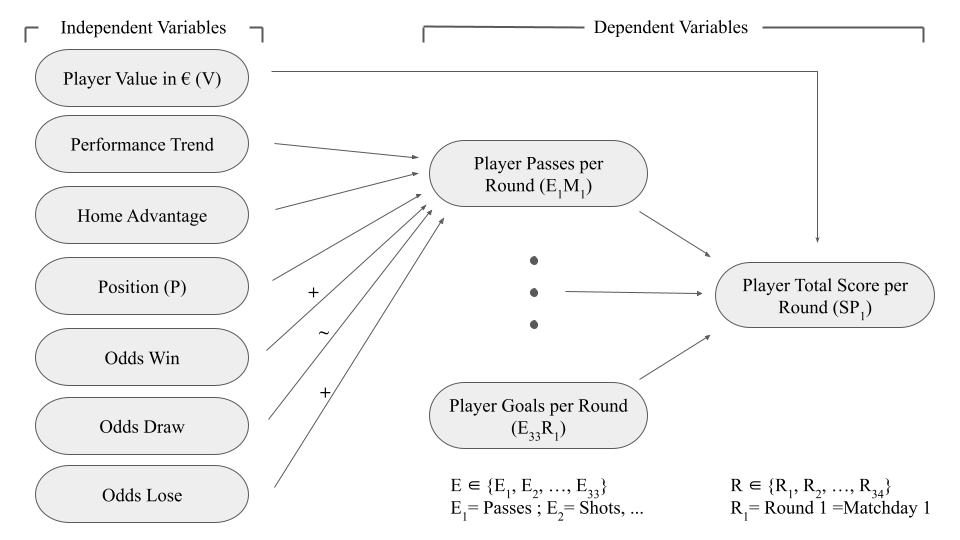
\includegraphics[width=15cm]{chapter/4_implementation/section/2_data/section/figures/variables.png}
    \captionsetup{justification=centering}
    \caption{Effects between Dependent and Independent Variables}
    \label{fig:dependent-independent}
\end{figure}



